\documentclass[10pt]{article}
%	options include 12pt or 11pt or 10pt
%	classes include article, report, book, letter, thesis
\usepackage[T1]{fontenc}
\usepackage[utf8]{inputenc}
\usepackage{graphicx}
\usepackage{authblk}
\usepackage{hyperref}
\usepackage{fullpage}
\usepackage{times}
\usepackage{capt-of}
\title{\textbf{Simulation Project --- 1}}
\author{Rahul Krishna}
\affil{North Carolina State University\\Email: \href{mailto:rkrish11@ncsu.edu}{rkrish11@ncsu.edu}\thanks{Source code: \url{https://github.com/rahlk/CSC579__Computer_Performance_Modeling}}}
\date{}

\begin{document}
\maketitle
\section*{Task 1}
\textit{Let us define the customer loss rate
 (CLR) as: CLR = $\frac{X}{N}$. Let the queue capacity K = 20. Plot the CLR against the value of
 $\rho$, for $\rho$ = 0.05 to $\rho$ = 0.95, in increments of 0.10. Submit two graphs: one for C = 1000 and one for C = 100000. Do you see any difference in the two plots? If so, can you explain the difference? If not, why do you think there is no difference? Explain your answer. Did you expect these results before running the experiment?\\}
 
 \begin{figure*}[ht!]
 \centering
 \begin{minipage}[]{0.48\linewidth}
  \centering
 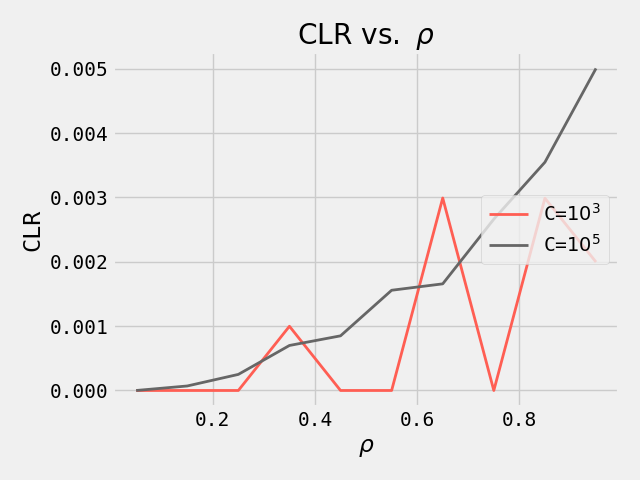
\includegraphics[width=\linewidth]{Figures/task1.png}
 \captionof{figure}{Customer loss rate v. $\rho$ for K=20}
 \label{fig1} 
 \end{minipage}~~~~\begin{minipage}  []{0.48\linewidth}
  \centering
  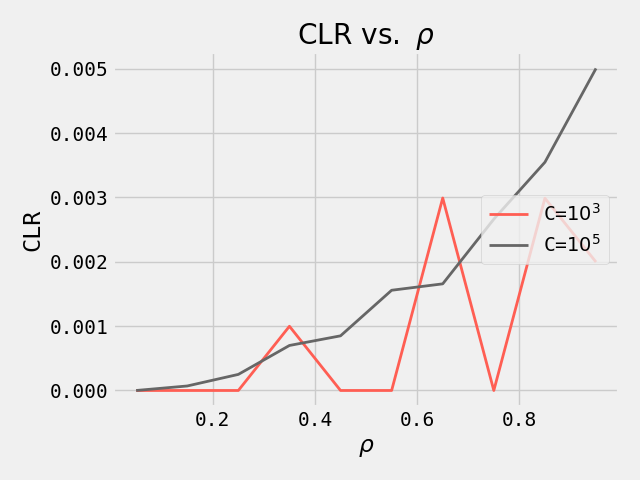
\includegraphics[width=\linewidth]{Figures/task1.png}
  \captionof{figure}{Customer loss rate v. $\rho$ for K=5}
  \label{fig2}
 \end{minipage}
\end{figure*}

 
 The plot of CLR against values of $rho$ for $\rho=0.05, 0.15,\ldots,0.95$ are shown in Fig. \ref{fig1}. 
 
 \begin{enumerate}
 
 \item This Fig indicates that the loss rate is 0 throughout the experiments for low values of $\rho$.This is because of the customer arrival time is exponentially distributed with rate $\lambda$ but the service time has a constant rate of $\mu=1$. This means that the customers are processed faster than they arrive. With a sufficiently large queue size (like K=20). There will be no dropped customers and thus CLR is 0.
 
 To verify if this is indeed the case, consider Fig. \ref{fig2}. Here K=5, and we see that with smaller queue, there are dropped customers are the arrival rate $\lambda$ approaches $\rho$.
 
 \item With K=20 (Fig. \ref{fig1}) we see no differences between the plots. This is because, once more, the queue size is large enough that even with $C=10^5$ served customers there are no losses. 
 
 Again, with K=5 (Fig. \ref{fig2}) we notice that there is a generally increasing trend $C=10^5$. The curves are much more smoother that with $C=1000$. This is because the $C=1000$ is too low to measure the loss rate.
 
 \item The results of Fig. \ref{fig1} were to be expected prior to simulation. Because, as mentioned previously, we were aware the K=20 was too big a queue size to loose any arriving customer. That's the reason K=5 was used to verify this.
 
 \end{enumerate}

\section*{Task 2}
\textit{Now let us fix $\rho = 0.85$. Plot the CLR against the value of the queue capacity K, as K increases from 10 to 100 in increments of 10. Explain the behavior of the plots as K increases, and especially, the rate of change in the CLR as a function of K . Is this expected? Also,explain any differences in the two graphs due to the length of each simulation run.} \\

The plots are shown in Fig. \ref{fig3} and Fig. \ref{fig4}

\end{document}

